\documentclass{article}
\usepackage[margin=1in]{geometry}
\usepackage{problemset}
\showsolntrue

% Custom commands
\newcommand{\R}{\mathbb{R}}
\newcommand{\X}{\mathcal{X}}
\newcommand{\Y}{\mathcal{Y}}
\newcommand{\E}{\mathbb{E}}
\newcommand{\V}{\text{Var}}
\renewcommand{\P}{\mathbb{P}}

\begin{document}

\pstitle{%
    MATH 189%
}{
    Homework 1%
}[due Wednesday, January 14 at 8:00AM]

\textbf{Resources:} These problems appear in Ch. 2 of the textbook pg. 63-67.

\textbf{Format requirements:} Type your homeworks using \LaTeX with embedded plots for the applied exercise.

\textbf{Grading:} The grading is based 50\% on correctness and 50\% on correctness.

\vspace{1em}

\begin{probset}

% --- Problem 1 ---
\begin{prob}[\textbf{Conceptual exercise 2}]
    Explain whether each scenario is a classification or regression problem, and indicate whether we are most interested in inference or prediction. Finally, provide $n$ and $p$.

    \begin{subprobset}
        \begin{subprob}
            We collect a set of data on the top 500 firms in the US. For each firm we record profit, number of employees, industry and the CEO salary. We are interested in understanding which factors affect CEO salary.

            \begin{soln}
                This is a regression problem because CEO salary is a continuous variable. We are interested in inference since we want to understand which factors affect CEO salary. $n = 500$ and $p = 3$ because there are 500 firms and 3 variables.
            \end{soln}
        \end{subprob}

        \begin{subprob}
            We are considering launching a new product and wish to know whether it will be a success or a failure. We collect data on 20 similar products that were previously launched. For each product we have recorded whether it was a success or failure, price charged for the product, marketing budget, competition price, and ten other variables.

            \begin{soln}
                This is a classification problem because the outcome is binary (success or failure). We are interested in prediction since we want to know whether the new product will be a success or a failure. $n = 20$ and $p = 13$ because there are 20 products and 13 variables.
            \end{soln}
        \end{subprob}
        
        \begin{subprob}
            We are interested in predicting the \% change in the USD/Euro exchange rate in relation to the weekly changes in the world stock markets. Hence we collect weekly data for all of 2012. For each week we record the \% change in the USD/Euro, the \% change in the US market, the \% change in the British market, and the \% change in the German market.

            \begin{soln}
                This is a regression problem because the exchange rate is a continuous variable. We are interested in prediction since we want to predict the exchange rate. $n = 52$ and $p = 3$ because there are 52 weeks and 3 variables.
            \end{soln}
        \end{subprob}
    \end{subprobset}
\end{prob}

\newpage

% --- Problem 2 ---
\begin{prob}[\textbf{Conceptual exercise 7}]
    The table below provides a training data set containing six observations, three predictors, and one qualitative response variable.

    \begin{center}
        \begin{tabular}{c|cccc}
            \hline
            Obs. & $X_1$ & $X_2$ & $X_3$ & $Y$ \\
            \hline
            1 & 2 & 0 & 0 & Red \\
            2 & 2 & 0 & 0 & Red \\
            3 & 0 & 1 & 3 & Red \\
            4 & 0 & 1 & 2 & Green \\
            5 & -1 & 0 & 1 & Green \\
            6 & 1 & 1 & 1 & Red \\
            \hline
        \end{tabular}
    \end{center}

    Suppose we wish to use this data set to make a prediction for $Y$ when $X_1 = X_2 = X_3 = 0$ using K-nearest neighbors.
    
    \begin{subprobset}
        \begin{subprob}
            Compute the Euclidean distance between each observation and the test point, $X_1 = X_2 = X_3 = 0$.

            \begin{soln}
                The Euclidean distance between each observation and the test point is:

                \begin{center}
                \begin{tabular}{|c|c|c|c|c|c|c|}
                    \hline
                    Obs. & 1 & 2 & 3 & 4 & 5 & 6 \\
                    Dist. & 2 & 2 & $\sqrt{10}$ & $\sqrt{5}$ & $\sqrt{2}$ & $\sqrt{3}$ \\
                    \hline
                \end{tabular}
                \end{center}
            \end{soln}
        \end{subprob}

        \begin{subprob}
            What is our prediction with $K = 1$? Why?

            \begin{soln}
                Since Obs. 5 has the smallest distance, our prediction is Green.
            \end{soln}
        \end{subprob}

        \begin{subprob}
            What is our prediction with $K = 3$? Why?

            \begin{soln}
                Since Obs. 5 Obs. 6, and Obs. 1 or 2 (both are red) have the smallest distances, our prediction is Red since we have 2 Red observations and 1 Green observation.
            \end{soln}
        \end{subprob}

        \begin{subprob}
            If the Bayes decision boundary in this problem is highly nonlinear, then would we expect the best value for $K$ to be large or small? Why?

            \begin{soln}
                If the Bayes decision boundary is highly nonlinear, then we would expect the best value for $K$ to be small because a small $K$ allows a more flexible, less-smoothed decision boundary that can adapt to nonlinearity.
            \end{soln}
        \end{subprob}
    \end{subprobset}
\end{prob}

\newpage

% --- Problem 3 ---
\begin{prob}[\textbf{Applied exercise 10}]
    This exercise involves the Boston housing data set.

    \begin{subprobset}
        \begin{subprob}
            To begin, load in the Boston data set, which is part of the ISLP library.

            \begin{verbatim}
from ISLP import load_data
Boston = load_data('Boston')
            \end{verbatim}
        \end{subprob}
        \begin{subprob}
            How many rows are in this data set? How many columns? What do the rows and columns represent?

            \begin{verbatim}
Boston.shape
            \end{verbatim}

            \begin{soln}
                There are 506 rows and 13 columns in this data set. The rows represent the suburbs of Boston and the columns represent the predictors.
            \end{soln}
        \end{subprob}

        \begin{subprob}
            Make some pairwise scatterplots of the predictors (columns) in this data set. Describe your findings.

            \begin{verbatim}
import seaborn as sns
sns.set_context("notebook", font_scale=2.0)
sns.pairplot(Boston)
            \end{verbatim}

            \begin{soln}
                \begin{center}
                    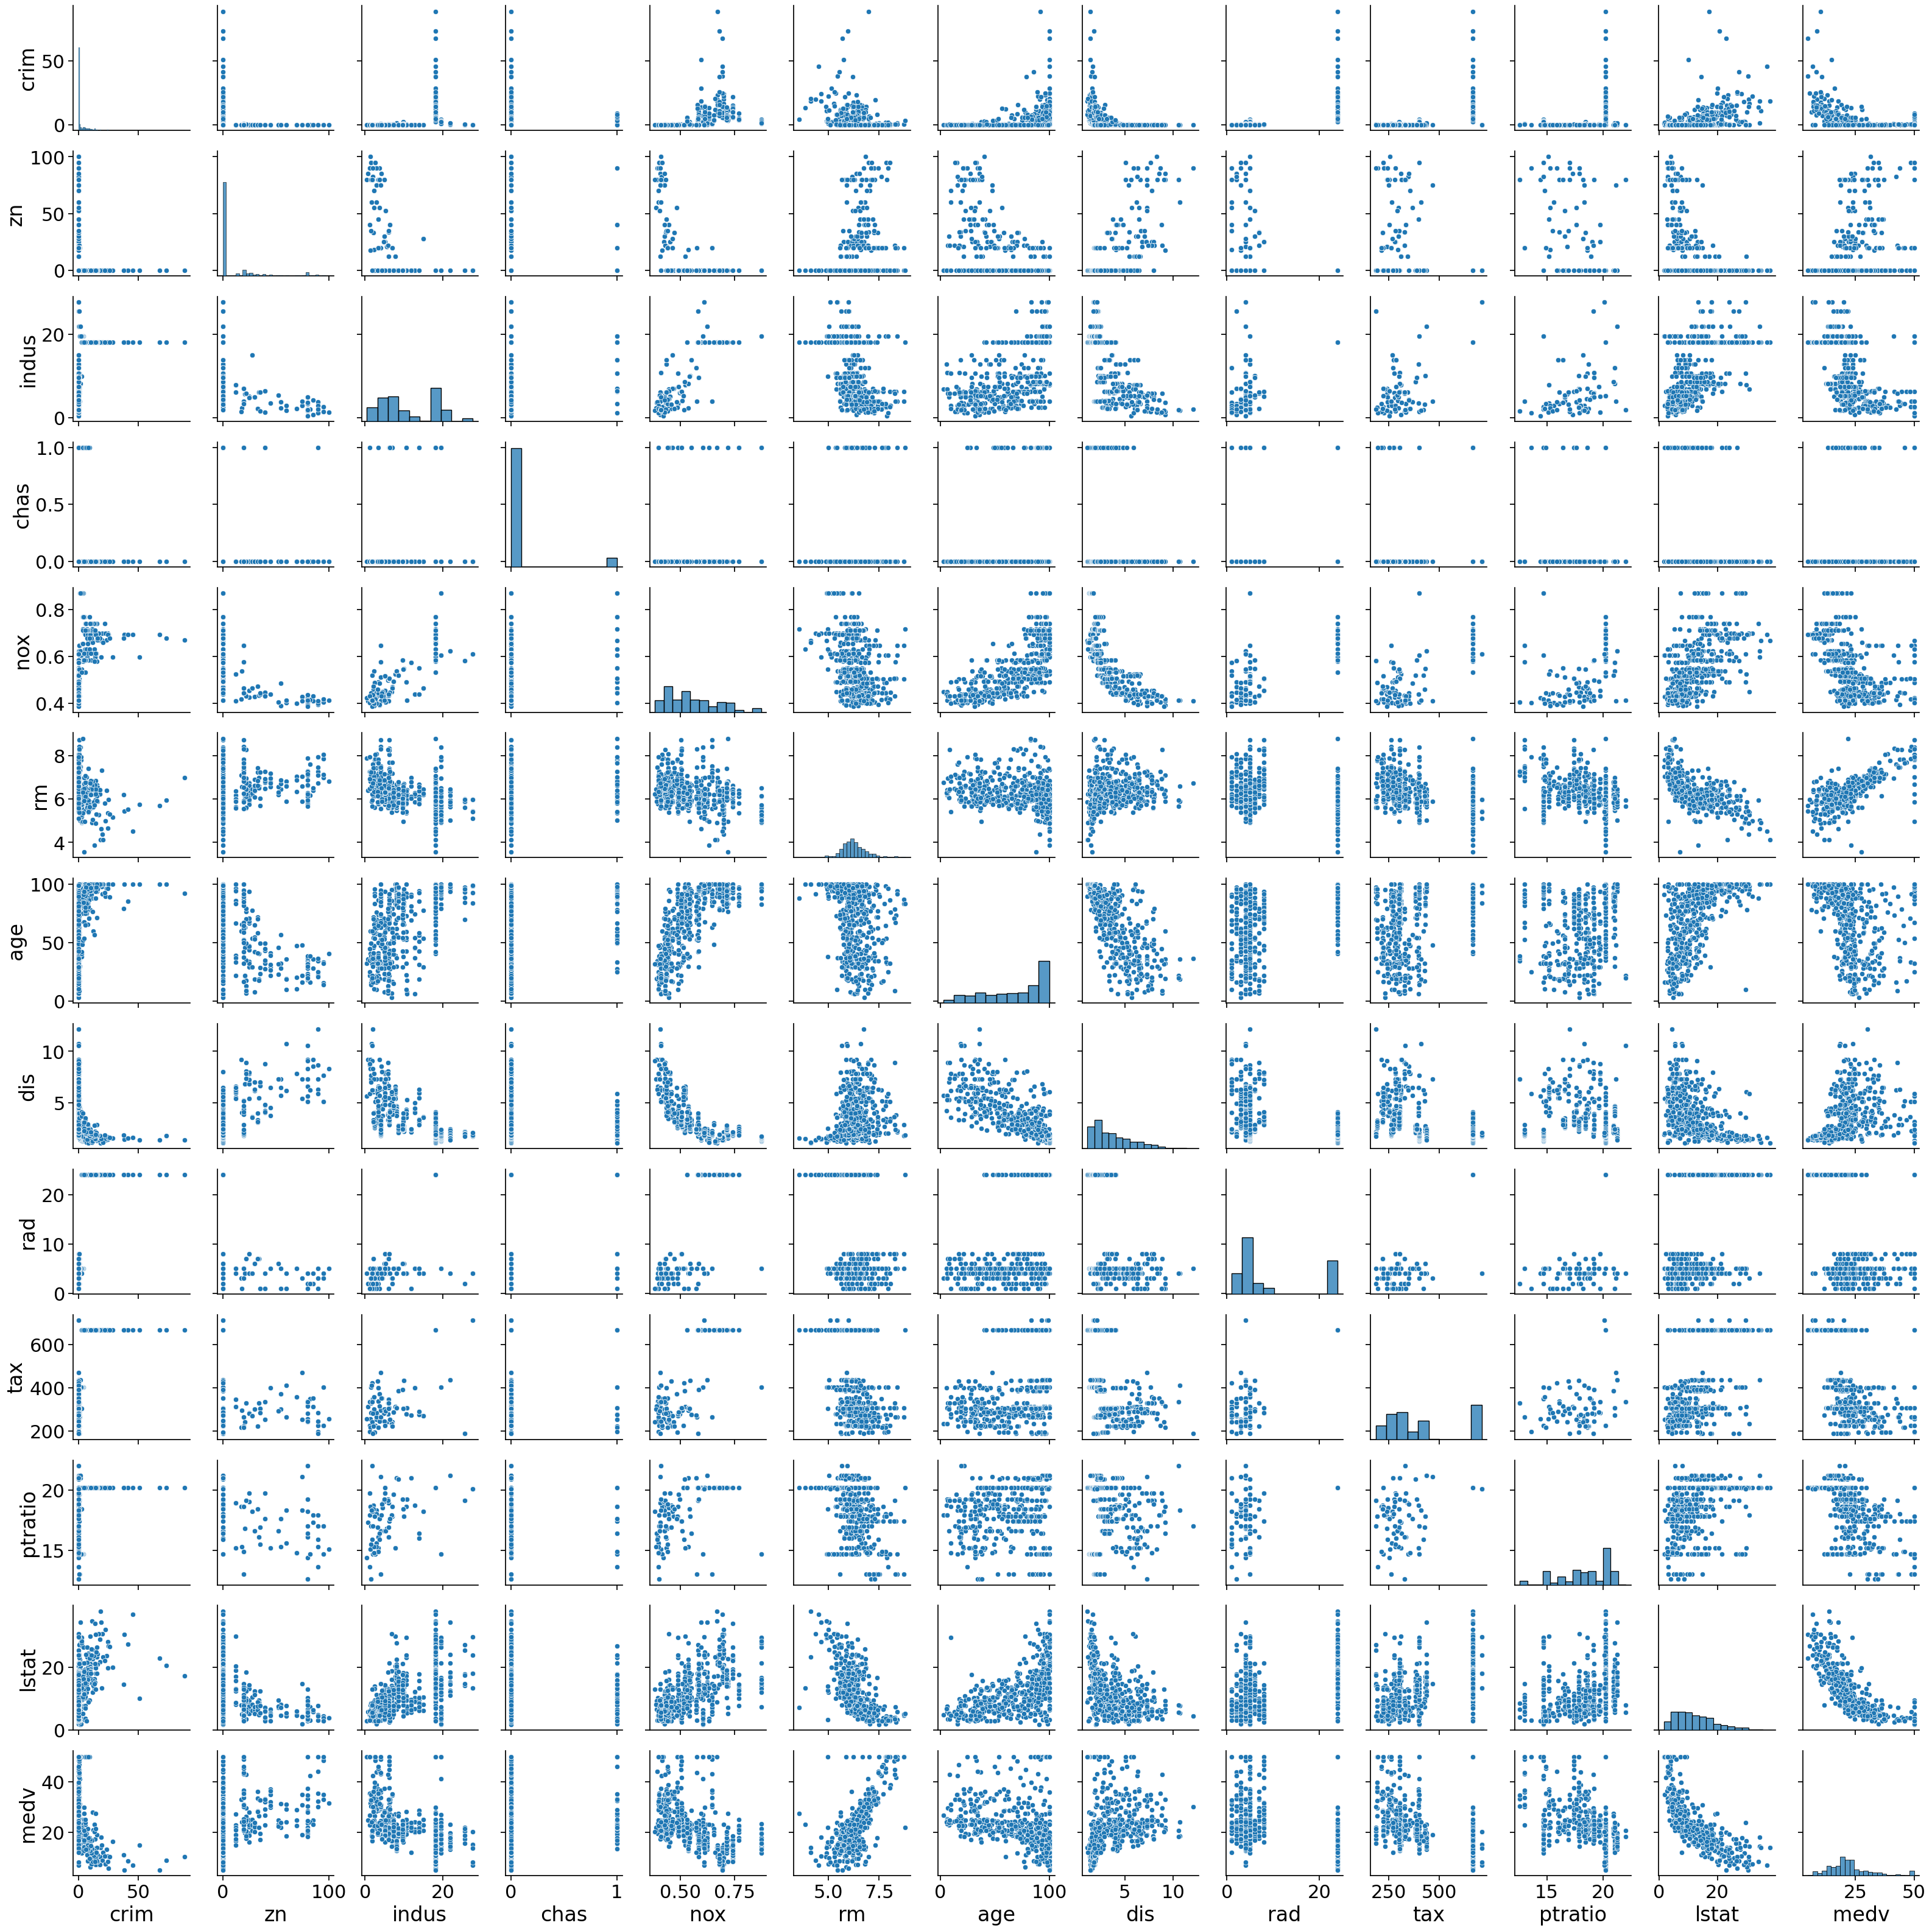
\includegraphics[width=0.7\textwidth]{Images/3.3.png}
                \end{center}
                Some of the strongest negative correlations are between \texttt{dis} and \texttt{age}, \texttt{indus}, and \texttt{nox}. Some of the strongest positive correlations are between \texttt{nox} and \texttt{age}, \texttt{indus}, \texttt{tax}.
            \end{soln}
        \end{subprob}

        \newpage

        \begin{subprob}
            Are any of the predictors associated with per capita crime rate? If so, explain the relationship.

            \begin{soln}
                \texttt{age} and \texttt{lstat} seems to be positively correlated with crime rate so as age increases, crime rate increases. Additionally, \texttt{dis} and \texttt{medv} seems to be negatively correlated with crime rate so as distance to employment centers increases, crime rate decreases.
            \end{soln}
        \end{subprob}

        \begin{subprob}
            Do any of the suburbs of Boston appear to have particularly high crime rates? Tax rates? Pupil-teacher ratios? Comment on the range of each predictor.

            \begin{verbatim}
Boston[["crim", "tax", "ptratio"]].describe()
            \end{verbatim}

            \begin{soln}
                Looking at the diagonal plots, we can see that most \texttt{crim} is around 0 with the 75th percentile being only at 3.68\% but there are a few suburbs with much higher crime rates as the max is 88.98\%. Additionally, looking at the scatterplots, we can see that \texttt{tax} has a bimodal distribution with peaks around 250 and 600. The min is 187 and the max is 711 for \texttt{tax}. Most suburbs have a \texttt{ptratio} are around 20 but a few are much lower with the min being 12.6 and the max being 22.0.
            \end{soln}
        \end{subprob}

        \begin{subprob}
            How many of the suburbs in this data set bound the Charles river?

            \begin{verbatim}
Boston[Boston["chas"] == 1].shape
            \end{verbatim}

            \begin{soln}
                There are 35 suburbs that bound the Charles river.
            \end{soln}
        \end{subprob}

        \begin{subprob}
            What is the median pupil-teacher ratio among the towns in this data set?

            \begin{verbatim}
Boston["ptratio"].median()
            \end{verbatim}

            \begin{soln}
                The median pupil-teacher ratio among the towns in this data set is 19.05.
            \end{soln}
        \end{subprob}

        \newpage

        \begin{subprob}
            Which suburb of Boston has lowest median value of owneroccupied homes? What are the values of the other predictors for that suburb, and how do those values compare to the overall ranges for those predictors? Comment on your findings.

            \begin{verbatim}
Boston[Boston["medv"] == Boston["medv"].min()]
            \end{verbatim}

            \begin{soln}
                The suburb of Boston with lowest median value of owner-occupied homes are suburbs 398 and 405 with a median value of 5.0. The \texttt{crim} values are relatively high for these suburbs compared to the overall range, being above 30\%. The \texttt{tax} values are also relatively high for these suburbs compared to the overall range, being above 600. The \texttt{ptratio} values are relatively average for these suburbs compared to the overall range, being around 20.
            \end{soln}
        \end{subprob}

        \begin{subprob}
            In this data set, how many of the suburbs average more than seven rooms per dwelling? More than eight rooms per dwelling? Comment on the suburbs that average more than eight rooms per dwelling.

            \begin{verbatim}
print("Number suburbs > 7 rooms per dwelling:", Boston[Boston["rm"] > 7].shape[0])
print("Number suburbs > 8 rooms per dwelling:", Boston[Boston["rm"] > 8].shape[0])

Boston[Boston["rm"] > 8].describe()
            \end{verbatim}

            \begin{soln}
                There are 64 suburbs that have more than 7 rooms per dwelling and 13 that have more than 8 rooms per dwelling. The \texttt{crim} values are relatively low for these suburbs compared to the overall range with the max being only 3.47\%. The distributions for \texttt{tax} and \texttt{ptratio} are relatively average similar to the overall distributions with smaller variances. Similarly, most other variables follow the overall distributions for these suburbs. One exception is \texttt{age} where the 25th percentile increased from 45 to 70.
            \end{soln}
        \end{subprob}
    \end{subprobset}
\end{prob}
\end{probset}
\end{document}
